\section{An Unbinned Fit of the Dijet Asymmetry}

The dijet asymmetry is defined as
\begin{equation}\label{eq:ResFit:Asymmetry}
  A = \frac{\pti{1'}-\pti{2'}}{\pti{1'}+\pti{2'}},
\end{equation}
where \pti{1'} and \pti{2'} refer to the randomly ordered \pt of the
leading two jets in an event.
In case of events with exactly two jets of same particle level jet
transverse momentum \pt and Gaussian response, the width $\sigma(A)$ of the asymmetry distribution is
related to the jet \pt resolution $\sigma$ by
\begin{equation*}
  \sigma(A) = \frac{1}{\sqrt{2}}\frac{\sigma}{\pt}.
\end{equation*}


\subsection{Dijet Pdf in Case of a Gaussian Response}

The dijet pdf~qeq{eq:ResFit:DijetPdf} is in fact equivalent to a pdf of the dijet
asymmetry with an additional assumption for the underlying particle
level jet spectrum, as will be shown in the following Sections.
The unbinned fitting method by maximisation of the
likelihood~qeq{eq:ResFit:Likelihood} has, however, certain advantages in
comparison to a more robust binned fit of the asymmetry
distribution.
For example, it enables an unambigous
determination of asymmetric response functions and a has high sensitivity to
extremely low populated regions of the response function.
These abilities are in particular important w.r.t. application in
the QCD background estimation for the SUSY search.
In this Note, a measurement only of a Gaussian response is discussed,
however.
\fixme{this has to be stated clearly in the intro}
Moreover, biases due to the event selection are explicitly considered
in the likelihood.
Therefore a better estimator of the particle level jet \pt is provided
as argument for the fitted resolution.
Finally, the response can in principle be measured simultaneosly
also for different event types, such as $\gamma+$jet events and in different
$\eta$ regions, thus increasing the covered $\pt$ range and the amount
of available events.

Additional acitivity in the events, e.g. from soft gluon radiation, as
well as out-of-cone effects during the jet clustering bias the dijet asymmery and have to be
corrected for when measuring the resolution.
It is discussed in detail in \qsec {sec:ResFit:AddJets}; the rest of
this Section is devoted to the comparison of the performance of a
binned and an unbinned fit of the dijet asymmetry.
The completely analogue case is demonstrated in
\qsec{sec:ResFit:Asym:SimpleFit} where the likelihood is simplified by replacing the spectrum
with the assumption \mbox{$\pttrue = \ptave$}.
Since the unbinned fit is more sensitive to non-Gaussian, an outlier
suppression technique is introduced.
In \qsec{sec:ResFit:Asym:FullFit}, the full dijet pdf, including an assumption for the
spectrum, is finally used to fit the asymmetry;
the spectrum is also used to derive a better estimator for \ptgen.

The dijet pdf~\qeq{eq:ResFit:DijetPdf} has been defined as a function
of \pti{1} and \pti{2}.
In what follows, the coordinates
\begin{eqnarray}
  \label{eq:ResFit:TransformedCoordinates}
  \Delta\pt & = & \frac{1}{2}\left(\pti{1}-\pti{2}\right) \\
  \ptave & = & \frac{1}{2}\left(\pti{1}+\pti{2}\right)
\end{eqnarray}
which are especially suited for a Gaussian response are being used.
With these coordinates, the dijet pdf~\qeq{eq:ResFit:DijetPdf} becomes
\begin{equation}
  \label{eq:ResFit:DijetPdfTransformed}
   g_{\sigma'}\left(\Delta\pt,\ptave\right) \propto
   \e^{-\frac{1}{2}\left(\frac{\Delta\pt}{\sigma'}\right)^{2}}
   \int^{\infty}_{0}\dif{\pttrue}\,f\left(\pttrue\right)
   \e^{-\frac{1}{2}\left(\frac{\ptave - \pttrue}{\sigma'}\right)^{2}}
\end{equation}



\subsubsection{Simple Maximum Likelihood Fit and Outlier Treatment}\label{sec:ResFit:Asym:SimpleFit}

If the spectrum in the dijet pdf is replaced by \mbox{$\pttrue =
  ptave$}, i.e. \mbox{$f(\pttue)  = \delta\left(\pttrue - \ptave\right)$},
\qsec{eq:ResFit:DijetPdfTransformed} simplifies to
\begin{equation}
\label{eq:ResFit::DijetPdfTransformed?Simple}
  g_{\sigama'}(\Delta\pt) \propto
  \e^{-\frac{1}{2}\left(\frac{\Delta\pt}{\sigma'}\right)^{2}}, 
\end{equation}
with \mbox{$\sigma' = \sigma/\sqrt{2}$}.
This corresponds to the pdf of the asymmetry in the event, assuming
Gaussian response.

In real data, however, there are non-Gaussian tails biasing the
Gaussian asymmetry fit.
In case of a binned fit, the influence of the tails is suppressed by
fitting only the Gaussian bulk of the asymmetry distribution.
In case of the unbinned fit described here, it is not as straight
forward to fit only the bulk events.
It can be achieved, however, with an iterative procedure by restricting
the allowed range of $\Delta\pt$.
From MC simulatin and data (\fixme{reference to plot}) it follows,
that the tails fall into the \pt range \mbox{$|\Delta\pt| > 2\sigma' =
  \frac{2}{\sqrt{2}}\sigma$}.
The unbinned fit is performed only for events with \mbox{$|\Delta\pt| < 2\sigma'$}.
In order to restrain unity of the dijet pdf, the normailisation
of~\qeq{eq:ResFit::DijetPdfTransformed:Simple} is adapted accordingly.
Varying the upper threshold, $2\sigma'$ during the fit, however, would
bias the result towards smaller \fixme{?} values.
Therefore the threshold is kept fixed and the maximisation iterated
four times, leading to an unbiased result.





\subsubsection{Full Maximum Likelihood Fit Including the Spectrum}\label{sec:ResFit:Asym:FullFit}


In the following, the prediction of the width of the asymmetry
distribution from the unbinned fit is compared to the result from a direct binned
fit to the asymmetry distribution.
In order to assure compatibility of the results, the dijet probability
density~\eqref{eq:qcd:resolMaxlike:dijetPdf} is simplified by assuming
\mbox{$\pttrue = \ptave$} in each event.
This prediction is in good agreement to the dijet asymmetry distribution
Fig.~\ref{fig:qcd:resolMaxlike:asymmetry} (left), measured in Collider
data in one example bin for \mbox{$140 < \ptave < 170\gev$}, \mbox{$\ppi{3}  < 
  0.1\cdot\mean{\pttrue}$}, and \mbox{$\ppi{\text{Soft}} < 
  0.015\cdot\mean{\pttrue}$}.
The predicted widths in different \ptave bins are further compared to
the widths of the direct binned Gaussian fits of the bulk of the asymmetry
distributions in Figure~\ref{fig:qcd:resolMaxlike:asymmetry} (right).
Again, there is good closure of the method.

In conclusion, the simplified likelihood fit performs equally to a
binned fit of the asymmetry distributions. 
The extension of the dijet probability density with an assumption for the particle
level jet \pt is discussed in the following; by this extension,
additionally a description of biases in the event selection can be
included into the likelihood and it is a neccessity in order to be
able to fit arbitrary, not necessarily Gaussian, response functions.


$\sqrt{2}$\\
State explicitly: asymmetry and resolution used as ``synonyms''


\begin{figure}[ht]
  \centering
  \begin{tabular}{cc}
%   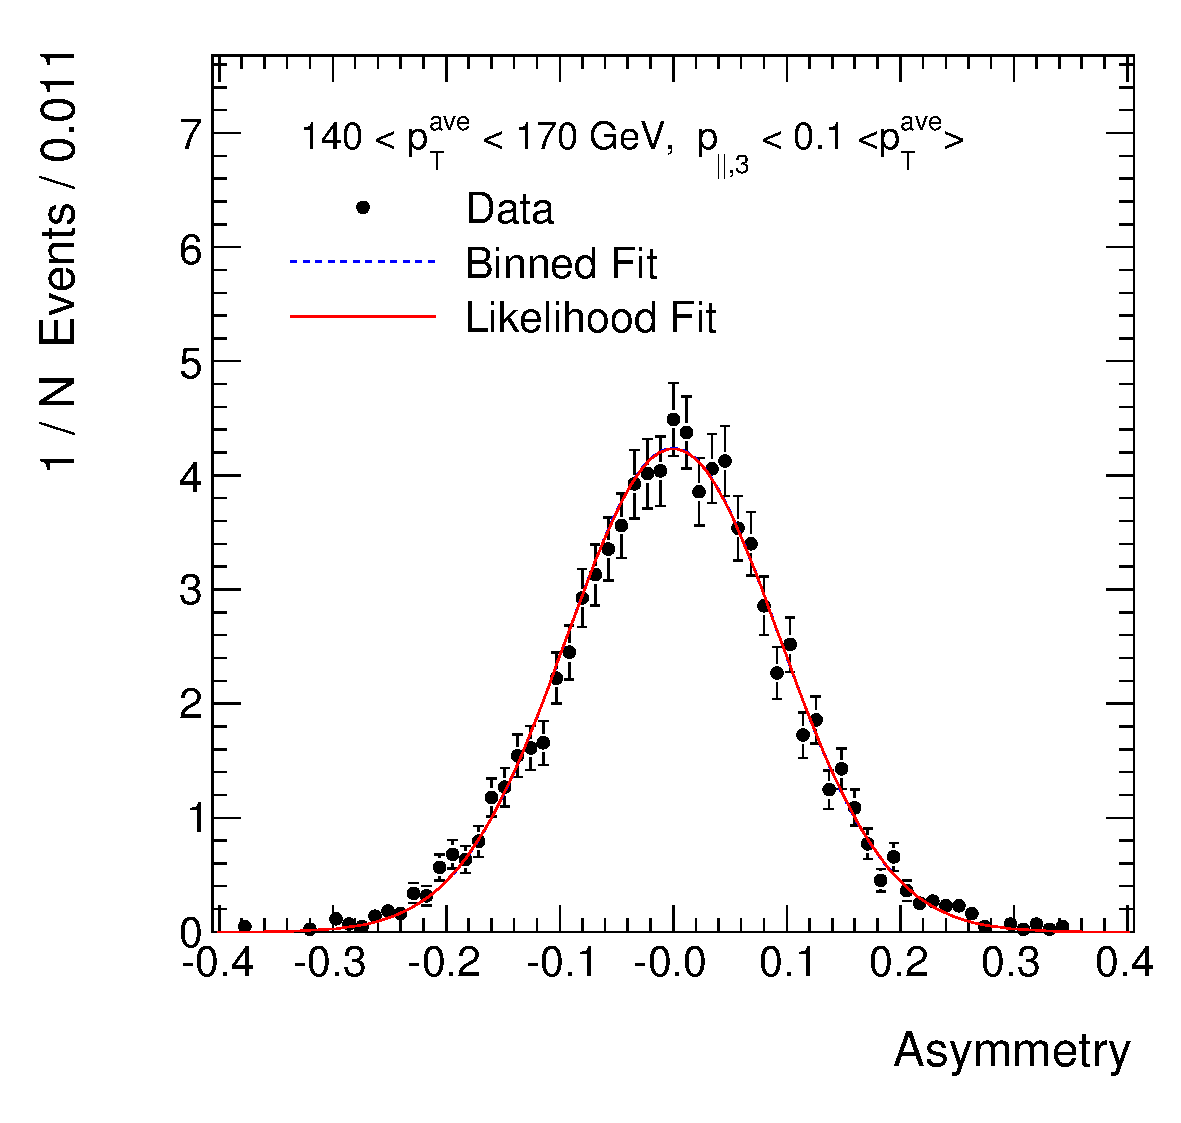
\includegraphics[width=0.45\textwidth]{figures/figures_QCD_resol_maxlike/MaxLikeSimple_Data132440-144011_Eta00-13_PtAsymmetry_PtBin4_Pt3Cut3} &
%    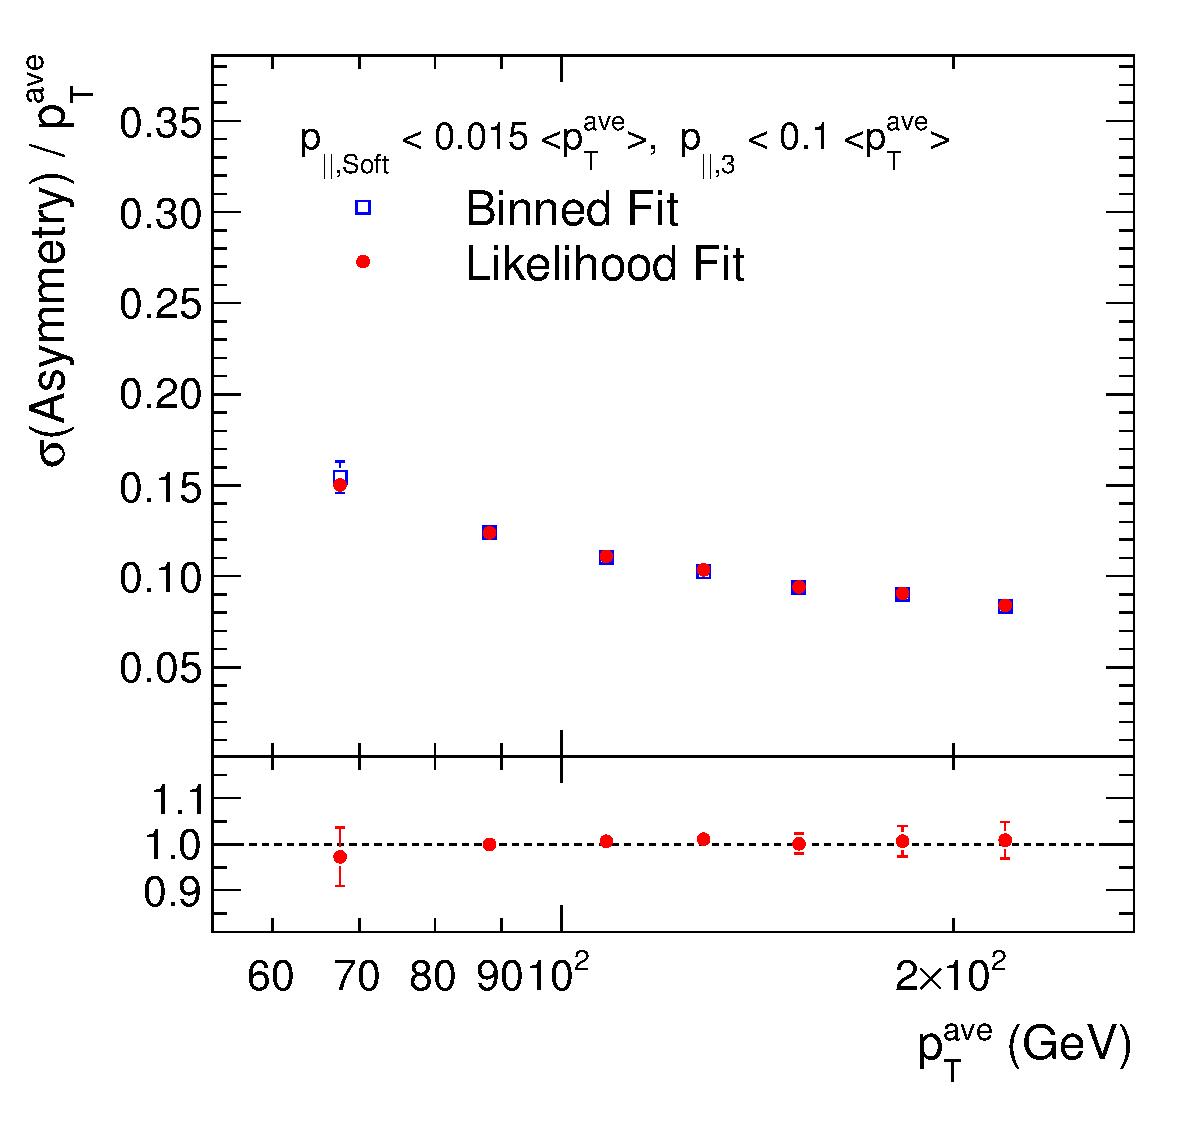
\includegraphics[width=0.45\textwidth]{figures/figures_QCD_resol_maxlike/MaxLikeSimple_Data132440-144011_Eta00-13_PtAsymmetryWidthBottomRatio_Pt3Cut3} \\
\end{tabular}
  \caption{(\textit{Left}) Dijet asymmetry distribution measured in
    Collider data (circles) for \mbox{$\ppi{3}  < 
      0.1\cdot\mean{\pttrue}$} in the \mbox{$140 < \ptave < 170\gev$} bin.
    It is well described by the prediction (solid line) from the
    simplified unbinned fit and there is good agreement to a direct binned
    Gaussian fit (dashed line) to the histogram.
    (\textit{Right}) Width of the asymmetry distributions from
    Collider data in different \ptave bins from binned Gaussian fits to the
    histograms (open squares) in comparison to the predictions from
    the unbinned fit (solid circles).}
  \label{fig:qcd:resolMaxlike:asymmetry}
\end{figure}



